\documentclass[10pt]{beamer}
\usepackage{tikz}
\usepackage{ifthen}
\usepackage[pdftex]{logopd}
\usepackage[absolute]{textpos}
\usetikzlibrary{snakes}
\usepackage{multimedia}
\usetheme[subsection=false]{DeiPadova}
\usecolortheme{Padova}
\usepackage{ulem}
\usepackage{tikz}
\usepackage[tikz]{mypics}
\usepackage{colortbl}
\usepackage{bm}
\usetikzlibrary{tikzmark,fit,shapes.geometric,arrows,graphs,plotmarks,patterns} %,graphdrawing}
\usepackage{mymaths}
\usepackage[beamer,short]{mybib}
\usepackage{epstopdf} 
\usepackage[linesnumbered,lined, algoruled]{algorithm2e}
\newcolumntype{R}[1]{>{\raggedleft\let\newline\\\arraybackslash\hspace{0pt}}m{#1}}

\newcolumntype{M}[1]{>{\centering\arraybackslash}m{#1}}

\AtBeginEnvironment{alertblock}{%
	\setbeamercolor{itemize item}{fg=alerted text.fg!50!black}
}
\AtBeginEnvironment{exampleblock}{%
	\setbeamercolor{itemize item}{fg=examplecol}
}
\setbeamercolor{math text}{fg=black}
%\usepackage{tabularx}
\usepackage{multirow}
%\usepackage{multicol}
\newcommand\pubkey[1]{\ensuremath{\C K_{\text{#1}}}}
\newcommand\privkey[1]{\ensuremath{k_{\text{#1}}}}
\newcommand\symkey[1]{\ensuremath{K_{\text{#1}}}}
\newcommand\cert[1]{\ensuremath{\text{cert}_{\text{#1}}}}
\usepackage{booktabs}
\newcommand\sgn{\mathop{\rm sgn}\nolimits}
\newcommand\mycite[3][alerted text.fg]{\textcolor{#1}{[#2, `#3]}}
\newcounter{nodemarkers}
\usepackage[acronym,shortcuts]{glossaries}

\newacronym{auc}{AUC}{area under the curve}
\newacronym{ap}{AP}{access point}
\newacronym{ce}{CE}{cross entropy}
\newacronym{cdf}{CDF}{cumulative distribution function}
\newacronym{fa}{FA}{false alarm}
\newacronym{kl}{K-L}{Kullback-Leibler}
\newacronym{ls}{LS}{least-squares}
\newacronym{llr}{LLR}{log likelihood-ratio}
\newacronym{los}{LOS}{line of sight}
\newacronym{lssvm}{LS-SVM}{least squares SVM}
\newacronym{md}{MD}{misdetection}
\newacronym{ml}{ML}{machine learning}
\newacronym{mlp}{MLP}{multy-layer perceptron}
\newacronym{mse}{MSE}{mean squared error}
\newacronym[\glslongpluralkey={neural networks}]{nn}{NN}{neural network}
\newacronym{np}{N-P}{Neyman-Pearson}
\newacronym{oclssvm}{OCLSSVM}{one-class least-square \ac{svm}}
\newacronym{pdf}{PDF}{probability density function}
\newacronym{pmd}{PMD}{probability mass distribution}
\newacronym{pso}{PSO}{particle swarm optimization}
\newacronym{rnn}{RNN}{replicator neural network}
\newacronym{roc}{ROC}{receiver operating characteristic}
\newacronym{roi}{ROI}{region of interest}
\newacronym{rss}{RSS}{received signal strength}
\newacronym[\glslongpluralkey={support vector machines}]{svm}{SVM}{support vector machine}
\newacronym{ue}{UE}{user equipment}
\newacronym{wsn}{WSN}{wireless sensor network}
\newacronym{irlv}{IRLV}{in-region location verification}

\newcommand{\cross}[2]{H_{#1}(#2)}
\newcommand{\hatcross}[2]{\hat{H}_{#1}(#2)}
\newcommand{\gy}{g(\bm a)}
%\newcommand{\E}[2]{\mathbb{E}_{#1}\left[#2\right]}
\newcommand{\pr}[1]{\mathbb{P} \left[ #1 \right]}

\title{Location-Verification and Network Planning \\ via Machine Learning Approaches}
\author[A. Brighente, \uline{F. Formaggio}, et al.]{A. Brighente, \underline{Francesco Formaggio}, M. Centenaro, G. M. Di Nunzio, and    S. Tomasin}
\vspace{1cm}
\institute[Department of Information Engineering, University of Padua]{\logopdred \hspace{1cm} \logodeinew  }
\date{}

%\AtBeginSection{\frame{\frametitle{Outline}\tableofcontents[currentsection]}}
%\logo{\begin{tikzpicture}[remember picture,overlay]
%    \node[xshift=-1.3cm,yshift=-7.3cm] at (current page.south){%
%    \includegraphics[width=0.55\textwidth]{Figure/logoENC.jpg}};
%\end{tikzpicture}}

\begin{document}
%\maketitle
\frame[plain]{\titlepage}
%\frame{\frametitle{Outline}\tableofcontents}

\begin{frame}{Motivation}
\begin{block}{Location aware services}
	Grant services only to users inside a certain physical area
\end{block}
\vspace{1cm}
\begin{itemize}
	\item Different from physical layer authentication
	\item Cannot use GPS: spoofing threat
	\item Do not want to make any assumption on channel model
\end{itemize}
\end{frame}	

\begin{frame}{Problem Statement}
\begin{columns}
	\column{0.5\textwidth}
	{ 	\fontsize{9}{9}
	\begin{block}{\Ac{irlv}}
			Decide whether a user is inside or outside the \ac{roi}
	\end{block}
}
\begin{itemize}
	\item Exploit location dependent channel features to discriminate physical areas \dots
	\item \dots collected by \acp{ap}
\end{itemize}
	\column{0.5\textwidth}
	\begin{figure}[]
		\centering
		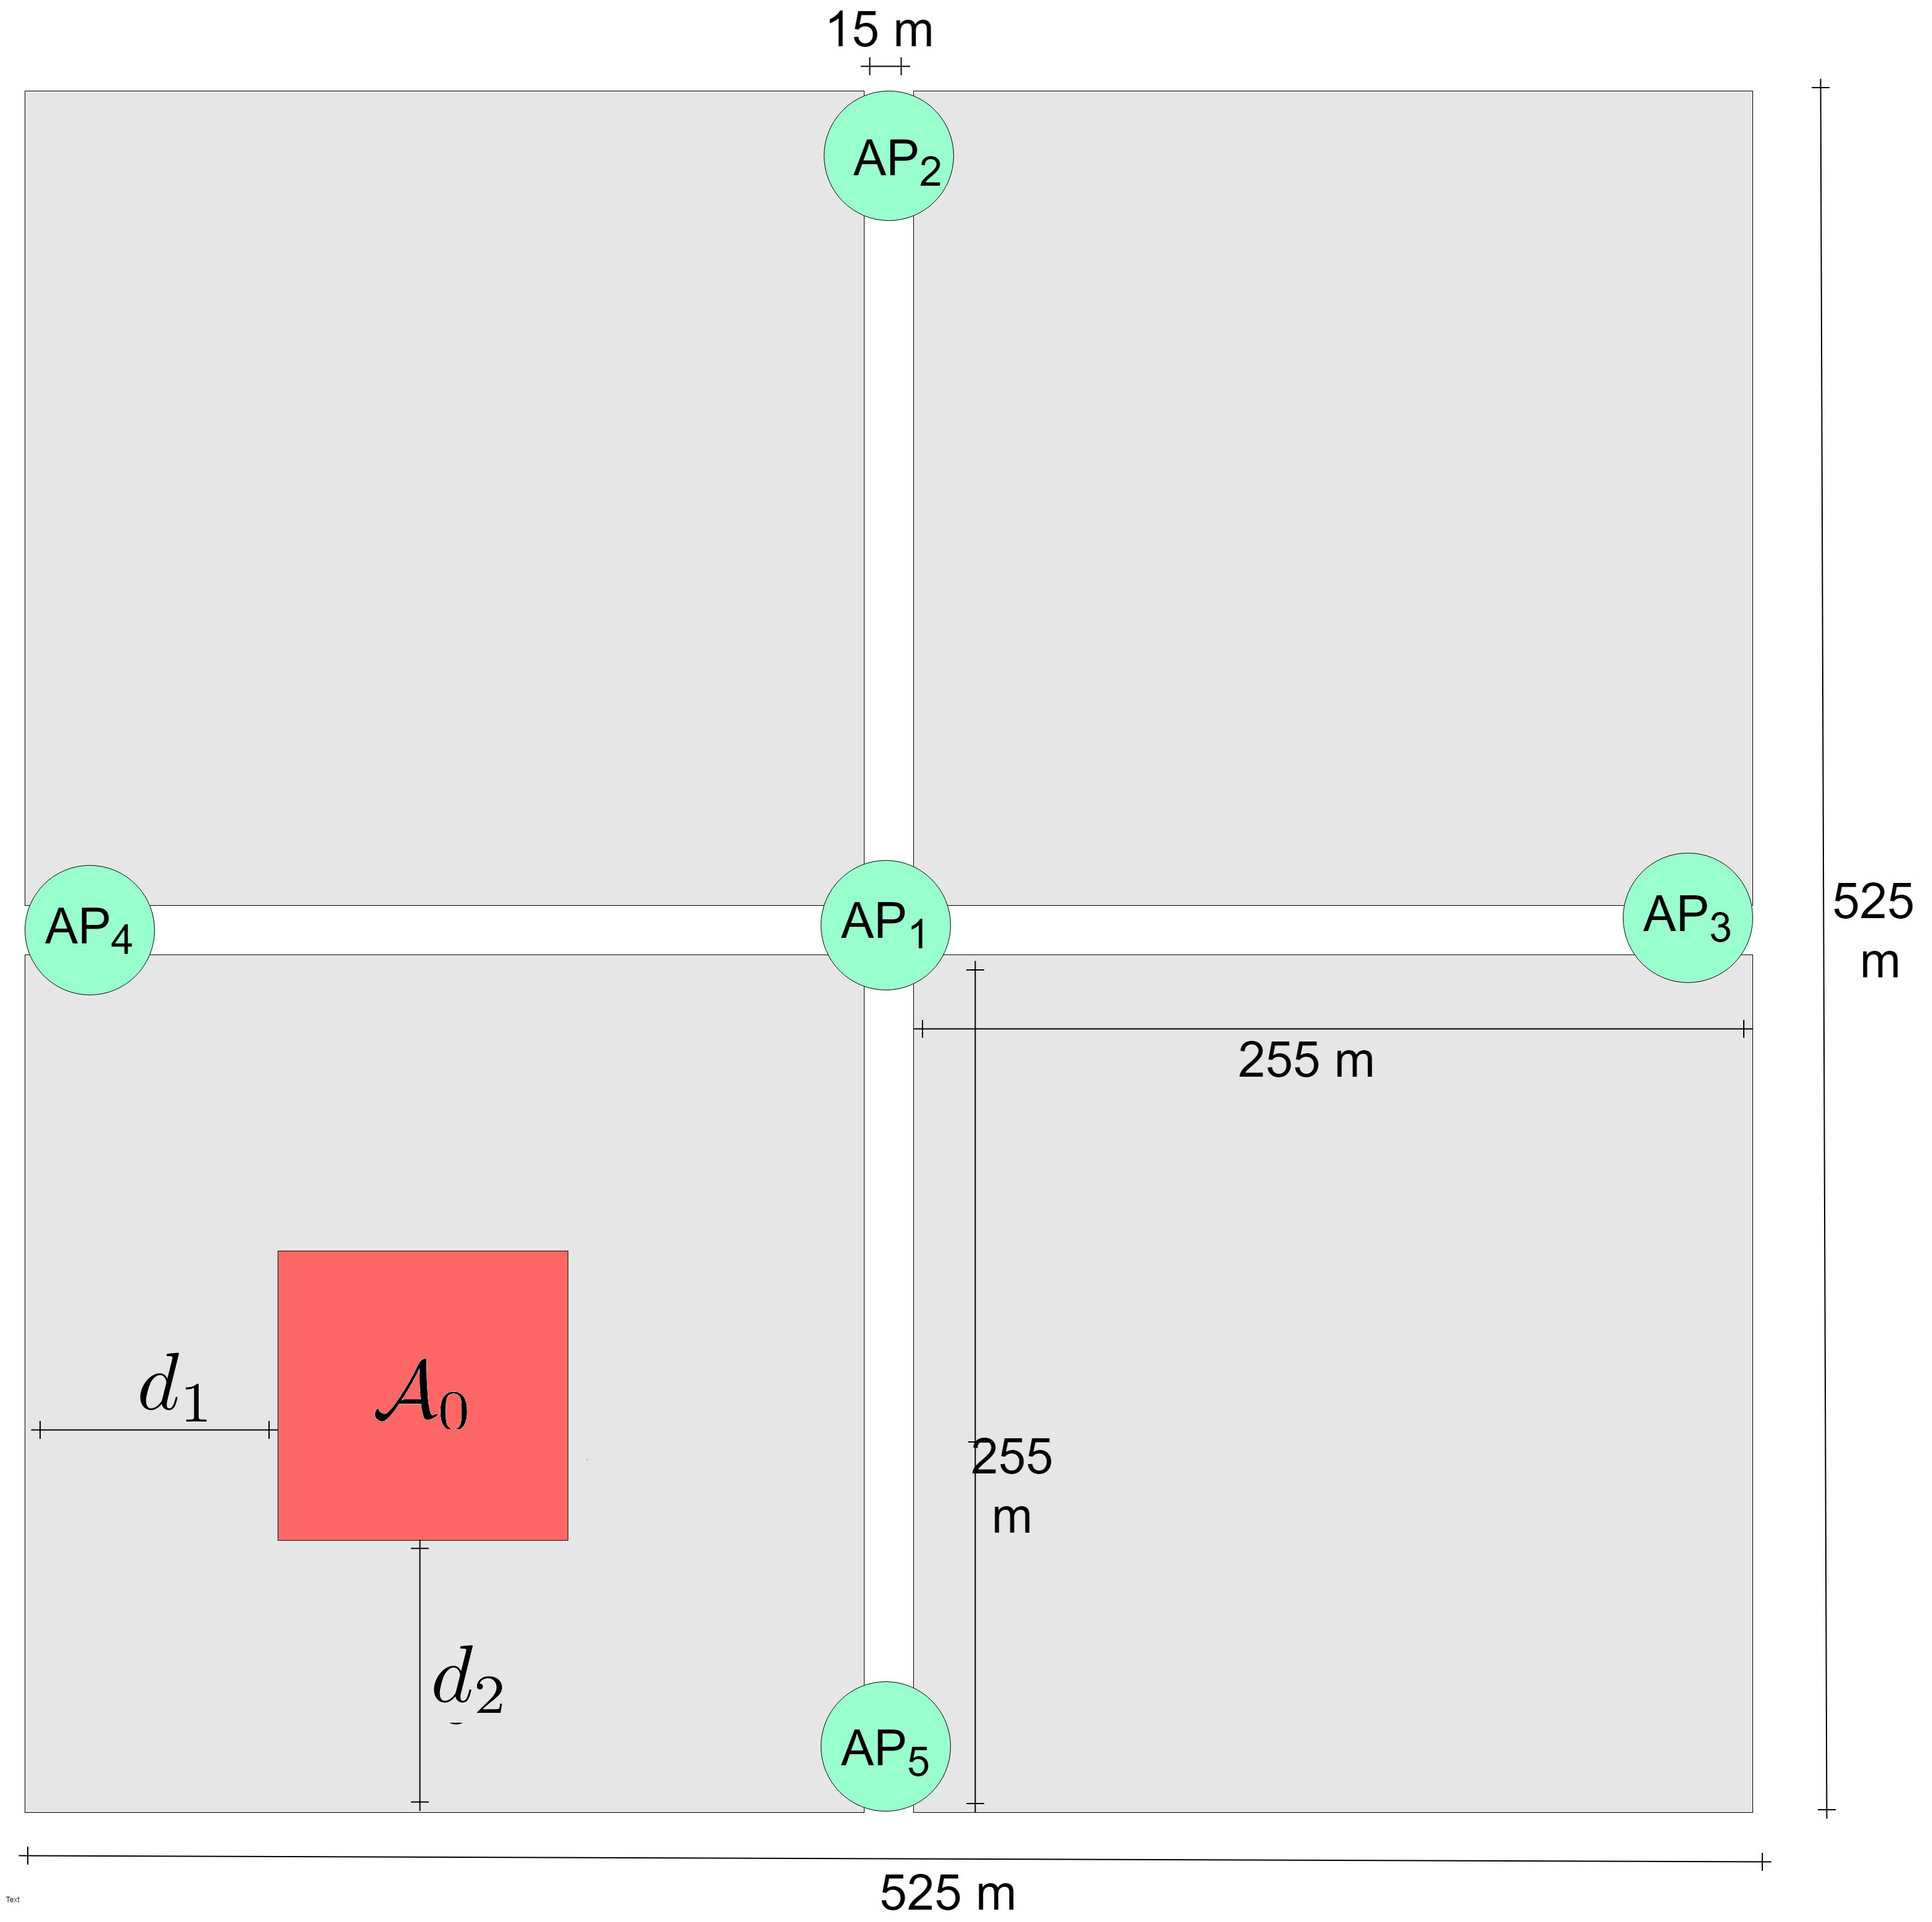
\includegraphics[width=1\columnwidth]{scenarioBuildingWiOpt.jpg}
	\end{figure}
\end{columns}
\end{frame}

\begin{frame}{Channel Model}
\begin{columns}
	\column{0.5\textwidth}
	\fontsize{9}{9}
	\begin{itemize}
		\item \acp{ap} attenuation values $$\bm{a}=[a(1),\ldots,a(N_{\rm AP})]$$
		\item Path-loss and shadowing
		\begin{equation*}
		\left(a{(n)}\right)_{\rm dB} = \left(a_{\rm PL}{(n)}\right)_{\rm dB} + \left(a_s{(n)}\right)_{\rm dB}
		\end{equation*}
		\item Log-normal shadowing:  
		$$\left(a_{\rm S}{(n)}\right)_{\rm dB} \sim \mathcal{N}(0,\sigma_s^2)$$ 
		\item \textbf{Spatial correlation}
%		 with decorrelation distance $d_c$:
%		\begin{equation*}
%		\E{\bm x}{a_{\rm S}(i)a_{\rm S}(j)} = \sigma_s^2\exp \left({-\frac{L(\bm{x}_i,\bm{x}_j)}{d_c}}\right).
%		\end{equation*}
	\end{itemize}
	\column{0.5\textwidth}
	\begin{figure}[t]
		\centering
		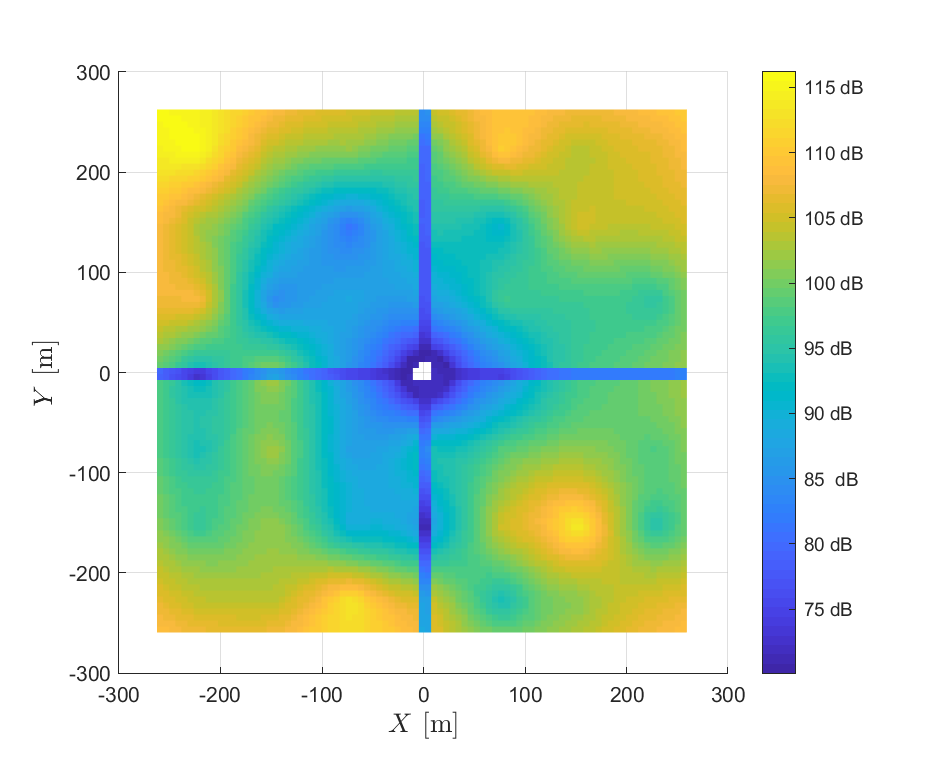
\includegraphics[width=\textwidth]{map.eps}
	\end{figure}
\end{columns}
\end{frame}

\begin{frame}{In-Region Location verification}
%\fontsize{9}{9}
\begin{itemize}
	\item Two hypotheses
	\begin{equation*}
	\hat{\mathcal{H}} = 
	\begin{cases}
	\mathcal{H}_0 \quad \text{User is inside } \mathcal{A}_0 \\
	\mathcal{H}_1 \quad \text{User is outside } \mathcal{A}_0
	\end{cases}
	\end{equation*}
\end{itemize}
	\begin{block}{Goal}
		Build a function $t(\bm{a})$ that maps attenuation vector $\bm a$ to its corresponding hypothesis
		\begin{equation*}
		\hat{\mathcal{H}} = t(\bm{a}) 
		\end{equation*}
	\end{block}
\begin{itemize}
	\item False alarm probability:
	$
	P_{\rm FA} =\pr{\hat{\mathcal{H}} =\mathcal{H}_1 | \mathcal H_0},
	$
	\item Mis-detection probability:
	$
	P_{\rm MD}=\pr{\hat{\mathcal{H}} =\mathcal{H}_1 | \mathcal H_1}. 
	$
\end{itemize}
\end{frame}

\begin{frame}{Known Attenuation Statistics}
\begin{itemize}
	\item \ac{irlv} as classical hypothesis testing between $\mathcal{H}_0$ and $\mathcal{H}_1$
	\item \ac{np} lemma provides minimum $P_{\rm MD}$ for a given $P_{\rm FA}$
	\item Compute the likelihood
	\begin{equation*}
	\mathcal{L}{(\bm a)}=\frac{p_{\bm a}(\bm a|\mathcal{H}_0)}{p_{\bm a}(\bm a|\mathcal{H}_1)}
	\end{equation*}
	\item For each threshold $\theta$ obtain optimum $(P_{\rm MD}, P_{\rm FA})$ couple
	\begin{equation*}
	\hat{\mathcal{H}} = t(\bm a) \triangleq \begin{cases}
	0 & \mathcal{L}{(\bm a)} \geq \theta\,, \\ 
	1 & \mathcal{L}{(\bm a)} < \theta 
	\end{cases}
	\end{equation*}
\end{itemize}
\end{frame}
\begin{frame}{Machine Learning Motivation}
	\begin{block}{Problem}
		\ac{np} requires known channel statistics
	\end{block}

\begin{itemize}
	\item Have to assume a channel (or  other features) model
	\item Hard to obtain analytical joint probability density  
\end{itemize}

\begin{block}{Solution}
	Let \ac{ml} techniques learn the channel statistics
\end{block}
\begin{itemize}
	\item \textbf{Identification phase}: collect labelled trusted attenuation values
	\item \textbf{Verification phase}: based on collected values classify new attenuation values
\end{itemize}
\end{frame}
\begin{frame}{Neural Network Implementation}
\begin{columns}
\column{0.5\textwidth}
%\fontsize{9}{9}
\begin{itemize}
%	\item Input $\bm{a}$ processed in stages $\to$ \emph{layers}
%	\item Output of each layer processed by scalar functions $\to$ \emph{neurons}
	\item Output of the $n^{\rm th}$ neuron of the $\ell^{\rm th}$ layer with weights $\bm{w}_n^{(\ell -1)}$ and bias $b_n^{(\ell)}$
	\begin{equation*}
	y_n^{(\ell)} = \sigma\left( \bm{w}_n^{(\ell -1)}\bm{y}^{(\ell-1)}+b_n^{(\ell)} \right) 
	\end{equation*}
	\item Empirical \ac{ce} between $g(\bm a)$ and labels $t_i$
	\begin{equation*}
%	\hatcross{p_{\mathcal{H}|\bm a}}{g}
	\begin{split}
  -\frac{1}{S}& \sum_{i=1}^{S}\bigg [t_i\log g(\bm a^{(i)}) + \\
	& +\left(1-t_i\right)\log\left(1-g(\bm a^{(i)})\right)\bigg ]
	\end{split}
	\end{equation*}
\end{itemize}
\column{0.5\textwidth}
% \centering
\def\layersep{1.5cm}

\begin{tikzpicture}[shorten >=1pt,->,draw=black!50, node distance=\layersep,scale=0.7]
\tikzstyle{every pin edge}=[<-,shorten <=1pt]
\tikzstyle{neuron}=[circle,fill=black!25,minimum size=17pt,inner sep=0pt]
\tikzstyle{input neuron}=[neuron, fill=green!50];
\tikzstyle{output neuron}=[neuron, fill=red!50];
\tikzstyle{hidden neuron}=[neuron, fill=blue!50];
\tikzstyle{annot} = [text width=4em, text centered]

% Draw the input layer nodes
\foreach \name / \y in {1,...,5}
% This is the same as writing \foreach \name / \y in {1/1,2/2,3/3,4/4}
\node[input neuron, pin=left:$a_\y$] (I-\name) at (0,-\y) {};

% Draw the hidden layer nodes
\foreach \name / \y in {1,...,6}
\path[yshift=0.5cm]
node[hidden neuron] (H-\name) at (\layersep,-\y cm) {};

% Draw the output layer node
\node[output neuron,pin={[pin edge={->}]right:$g(\bm{a})$}, right of=H-3] (O) {};

% Connect every node in the input layer with every node in the
% hidden layer.
\foreach \source in {1,...,5}
\foreach \dest in {1,...,6}
\path (I-\source) edge (H-\dest);

% Connect every node in the hidden layer with the output layer
\foreach \source in {1,...,6}
\path (H-\source) edge (O);

% Annotate the layers
\node[annot,above of=H-1, node distance=1cm] (hl) {Hidden layers};
\node[annot,left of=hl] {Input layer};
\node[annot,right of=hl] {Output layer};
\end{tikzpicture}

\end{columns}
\end{frame}

\begin{frame}{Optimality of Neural Network}
%\fontsize{9}{9}

\begin{block}{Theorem}
	Assumptions
	\begin{itemize}
		\item $\gy \in [0,1]$ \ac{nn} soft output
		\item \ac{ce} training
		\item Perfect training
	\end{itemize}
Then
%Let $\gy \in [0,1]$ be the output of a \ac{nn} obtained with perfect training, i.e., with infinite number of training points, layers and neurons. Let the training be performed with the \ac{ce} metric. Then
\begin{equation*}
\gy = p_{\mathcal H|\bm a}(\mathcal{H}_0|\bm a)	
\end{equation*}
almost surely
\end{block}
\begin{itemize}
\item At convergence: \ac{nn} performance $\to$ \ac{np} performance
\item \ac{nn} advantage: does not require input statistics during training
\end{itemize}
\end{frame}

\begin{frame}{Network Planning}
\begin{itemize}
\item \textbf{Observation}. Attenuation depends on position of \acp{ap} and surrounding environment 
\item Need to optimize \acp{ap} positions
\item \textbf{Security metric}. \Ac{roc} \ac{auc}
\begin{equation*}
C(\{\bm{x}_{\rm AP}^{(n)}\})  \triangleq \int_{0}^{1} P_{\rm MD}\left(P_{\rm FA}\right) d P_{\rm FA},
\end{equation*}

\end{itemize}
\begin{block}{Network Planning}
\begin{itemize}
\item Problem: find optimal location of \acp{ap}
\item Solution: \ac{pso}
\end{itemize}
\end{block}
\end{frame}

\begin{frame}{Particle Swarm Optimization}
\begin{columns}
\column{0.5\textwidth}
\begin{itemize}
\item Iterative algorithm 
\item Particle $\triangleq$ set of \acp{ap} position
\item One value of objective function  $\mathcal{B}_p$ for each particle
\item At each iteration update particles locations and velocities in the direction of the best solutions
\item In our case $\mathcal{B}_p \triangleq$ \ac{roc} \ac{auc}
\end{itemize} 


\column{0.5\textwidth}
\fontsize{9}{9}
\begin{algorithm}[H]

\tiny

\KwData{ number of particles $P$, $N_{\rm AP}$}
\KwResult{optimal position }
Initialize particles\;
train the \ac{nn} algorithm for each particle\;
$\mathcal{B}_p^{(0)}$, $p=1,\ldots,N_p$\;
$\mathcal{B}_g=\underset{p=1,\ldots,N_p}{\min} \, \mathcal{B}_p^{(0)}$\;
$i = 0$\;

\Repeat{convergence of $\mathcal{B}_g$}{
$i = i + 1$\;
\For{$p=1,\ldots,P$}{
update velocity and position vector of particle\;
train the \ac{nn} for each particle $\to$ $\mathcal{B}_p^{(i)}$\;
\If{$\mathcal{B}_p^{(i)} < \mathcal{B}_g$}{ $\mathcal{B}_g = \mathcal{B}_p^{(i)}$ \;}
}

}
\end{algorithm}     
\end{columns}

\end{frame}

\begin{frame}{PSO Objective Function}
Each \ac{pso} iteration requires
\begin{itemize}
	\item \ac{nn} training
	\item \ac{nn} testing
	\item \ac{roc} \ac{auc} computation
\end{itemize}

\begin{block}{Observation}
	Use cross-entropy as \ac{roc} \ac{auc} proxy
\end{block}
\begin{itemize}
\item Set $\mathcal{B}_p \triangleq$ \ac{ce}$_p$
\item \ac{ce} readily available after training
\end{itemize}   
\end{frame}

\begin{frame}{Simulations: NN optimality}
\begin{columns}
	\column{0.5\textwidth}
	\begin{figure}[]
		\centering
	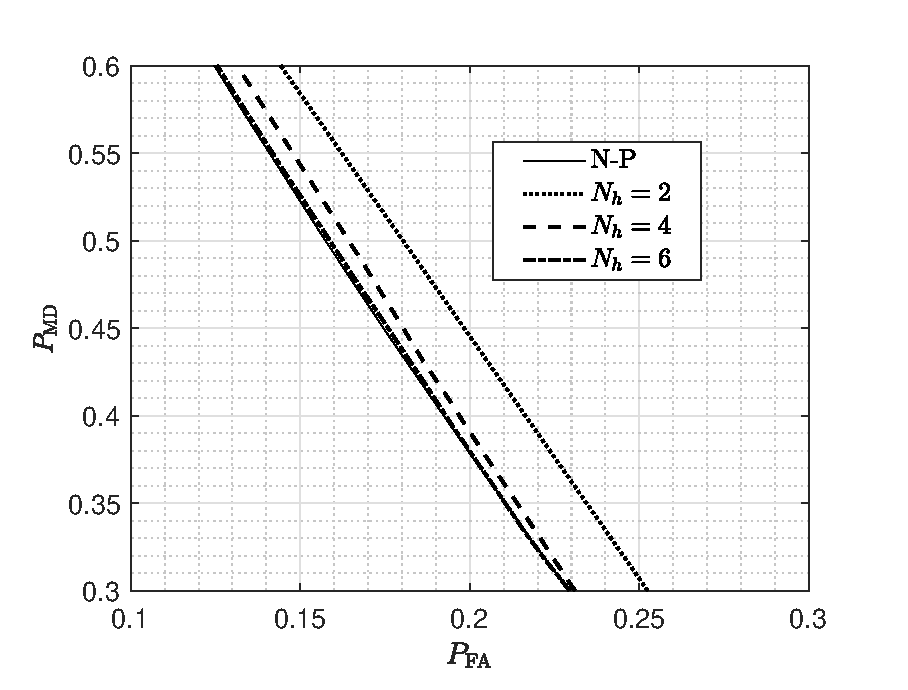
\includegraphics[width=1\columnwidth]{FA_MD_LOS.eps}
	\end{figure}
	\column{0.5\textwidth}
	\begin{itemize}
		\item Simple scenario with only one \ac{ap}
		\item Can compute \ac{np} likelihood ratio
		\item Higher \ac{nn} complexity (number of layers $N_h$) yields convergence to \ac{np}
	\end{itemize}
\end{columns}
\end{frame}

\begin{frame}{Training Convergence}
\begin{columns}
\column{0.5\textwidth}
\begin{figure}[]
\centering
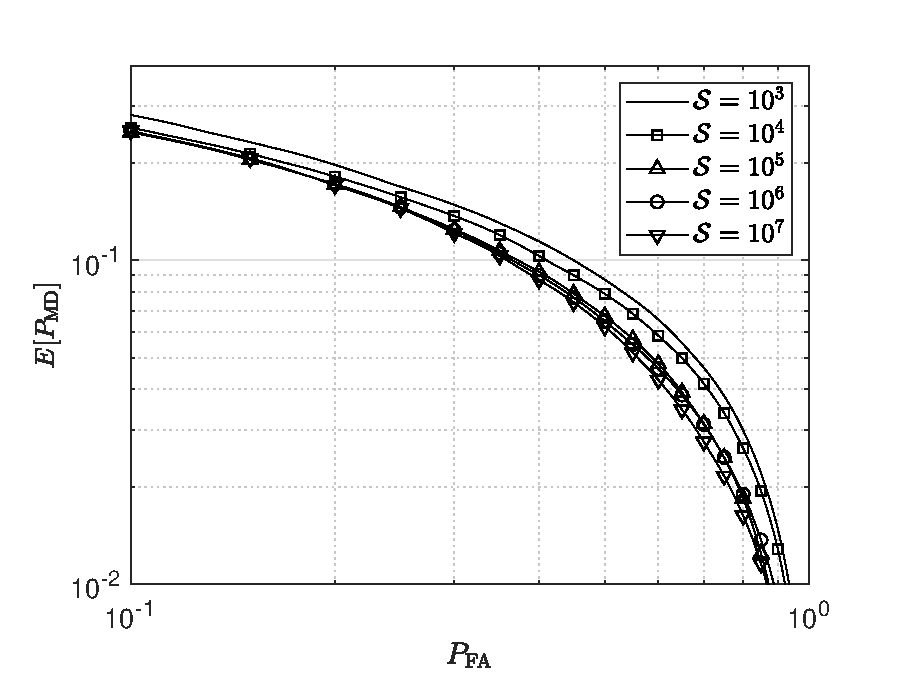
\includegraphics[width=1\columnwidth]{res_avg_nTrain.eps}
\label{fig:n_train}
\end{figure}
\column{0.5\textwidth}
\begin{itemize}
\item Average $P_{\rm MD}$ vs. $P_{\rm FA}$
\item Different number of training points $S$
\item Three layers with $8$ neurons in the hidden layer
\item Fully connected \ac{nn}
\item After $S=10^5$ performance do not improve \footnote[frame]{Brighente, Formaggio, et al., \textit{Machine Learning For In-Region Location Verification In Wireless Networks}, accepted for publication in IEEE JSAC}
\end{itemize}
\end{columns}
\end{frame}

\begin{frame}{Network Planning Performance}
\begin{columns}
\column{0.5\textwidth}
\begin{figure} 
\centering
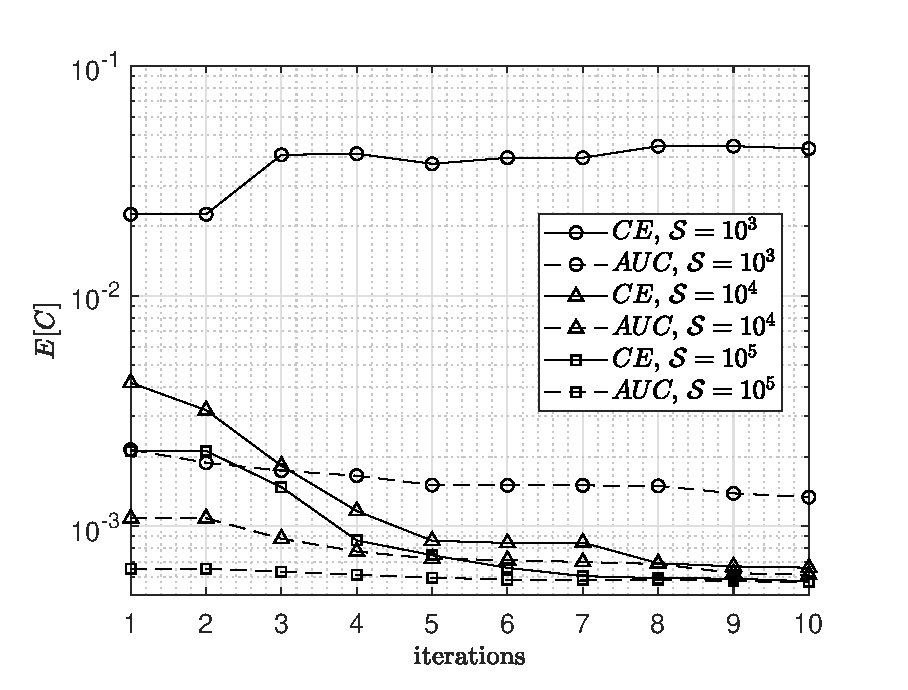
\includegraphics[width=1\columnwidth]{res_PSO_comp.eps}
\end{figure}
\column{0.5\textwidth}
\begin{itemize}
\item Mean \ac{auc} vs. number of iterations
\item Comparison between \ac{ce} and \ac{auc} minimization in \ac{pso}
\item \ac{ce} is a good proxy for \ac{auc} for a sufficient number of training points
\end{itemize}
\end{columns}
\end{frame}

\begin{frame}{Conclusions}
\begin{itemize}
\item \ac{irlv} as hypothesis testing problem
\item Novel \ac{nn}-based solution
\item Established connection between \ac{np} and \ac{nn} classification
\item Proposed a security-driven algorithm for network planning
\item \ac{ce} can be used as proxy of the \ac{auc}
\end{itemize}
\end{frame}

\begin{frame}{Questions?}
	Thank you for your attention
\end{frame}

\end{document}
